\titledquestion{Meeting the Bound}

\textbf{Meeting the Bound}

Consider binary trees of integers:

\begin{codeblock}
  datatype tree = Empty | Node of tree * int * tree
\end{codeblock}

A \textit{root-to-leaf path} is the sequence of values encountered walking from
the root down to an \code{Empty}. The \textit{weight} of a path is the sum of
those values. We are interested in the maximum weight over all root-to-leaf
paths.

For example, in the tree

\begin{center}
  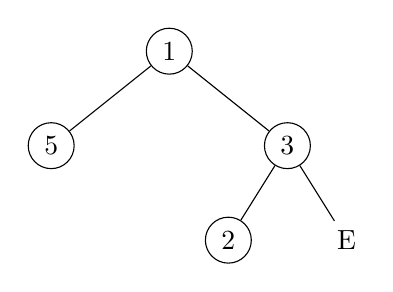
\begin{tikzpicture}[
    level 1/.style={sibling distance=30mm},
    level 2/.style={sibling distance=15mm},
    level distance=12mm,
    circ/.style={draw=black, circle, inner sep=3pt}
  ]
    \node[circ] {1}
      child{node[circ] {5}}
      child{node[circ] {3}
        child{node[circ] {2}}
        child{node {\code{E}}}
      }
    ;
  \end{tikzpicture}
\end{center}

the root-to-leaf paths have weights $1 + 5 = 6$ and $1 + 3 + 2 = 6$ and
$1 + 3 = 4$, so the maximum is $6$.

Throughout this problem, let $n$ be the number of \code{Node}s in the tree, and
let $d$ be its depth.

\begin{parts}
  \part[4]\hfill

    A student proposes the following implementation. It first computes the total
    sum of a subtree, then descends into whichever subtree has the larger total.

    \begin{codeblock}
      fun sumAll Empty = 0
        | sumAll (Node (L, x, R)) = x + sumAll L + sumAll R

      fun maxPath Empty = 0
        | maxPath (Node (L, x, R)) =
            if sumAll L > sumAll R then
              x + maxPath L
            else
              x + maxPath R
    \end{codeblock}

    This implementation is not merely slow --- it is \textbf{wrong}. Give a
    tree on which it returns an incorrect answer, and state both what it
    returns and what the correct answer is.

    \begin{solutionorbox}[16em]
      Consider:
      \begin{codeblock}
        Node ( Node (Node (Empty,4,Empty), 4, Node (Empty,4,Empty)),
               0,
               Node (Empty, 9, Empty) )
      \end{codeblock}

      The left subtree has total sum $12$, the right has total sum $9$, so the
      code descends left and returns $0 + 4 + 4 = 8$.

      But the best path goes right: $0 + 9 = 9$. The correct answer is $9$.

      The error is that a subtree with a large \textit{total} need not contain
      the best single \textit{path}.
    \end{solutionorbox}

  \newpage

  \part[8]\hfill

    Implement \code{maxPath} correctly, subject to a cost bound.

    \spec
      {maxPath}
      {\code{tree -> int}}
      {\code{true}}
      {\code{maxPath T} $\eeq$ the maximum weight over all root-to-leaf paths
      in \code{T}, and \code{0} when \code{T} $\eeq$ \code{Empty}}

    \begin{constraint}
      Your implementation must have work $W(n) = O(n)$.
    \end{constraint}

    \begin{solutionorbox}[16em]
      \begin{codeblock}
        fun maxPath Empty = 0
          | maxPath (Node (L, x, R)) =
              x + Int.max (maxPath L, maxPath R)
      \end{codeblock}

      Each node is visited exactly once, and the answer is built bottom-up
      rather than by recomputing subtree information at every level.
    \end{solutionorbox}

  \part[5]\hfill

    Write and solve a recurrence for the \textbf{work} of your implementation,
    in terms of $n$. You may assume the tree is roughly balanced.

    \begin{solutionorbox}[18em]
      $W(0) = c_0$

      $W(n) = c_1 + 2W(n/2)$

      Drawing the recursion tree: level $i$ has $2^i$ nodes each doing $O(1)$
      work, and there are $\log n$ levels, giving
      $\sum_{i=0}^{\log n} 2^i = O(n)$.

      So $W(n) = O(n)$, meeting the required bound: every node contributes
      $O(1)$ work and each is visited once.
    \end{solutionorbox}

  \newpage

  \part[5]\hfill

    Write and solve a recurrence for the \textbf{span} of your implementation,
    in terms of the depth $d$.

    Then explain, in one or two sentences, what property of your code makes
    this span achievable.

    \begin{solutionorbox}[20em]
      $S(0) = c_0$

      $S(d) = c_1 + S(d - 1)$

      which solves to $S(d) = O(d)$.

      This is achievable because the two recursive calls \code{maxPath L} and
      \code{maxPath R} are \textbf{independent}: neither takes the other's
      result as input, so they may be evaluated in parallel. The span therefore
      follows a single root-to-leaf path rather than summing over all nodes.

      (Contrast the first student's code, where \code{sumAll L} must complete
      before the branch is chosen --- introducing a dependency that the
      correct version does not have.)
    \end{solutionorbox}

  \part[4]\hfill

    Now suppose we switch to \textit{rose} trees, where a node may have any
    number of children:

    \begin{codeblock}
      datatype rose = Rose of int * rose list
    \end{codeblock}

    A root-to-leaf path now ends at a \code{Rose} with no children.

    Implement \code{maxPathRose : rose -> int}, still with work $O(n)$.

    \textbf{For this part, and only this part, pretend that \code{List.map}
    runs each of its calls in parallel.} Under that assumption, state the span
    of your implementation in terms of the depth $d$ and the maximum number of
    children $k$.

    \begin{solutionorbox}[22em]
      \begin{codeblock}
        fun maxPathRose (Rose (x, [])) = x
          | maxPathRose (Rose (x, cs)) =
              x + foldl Int.max
                    (~(valOf Int.maxInt))
                    (List.map maxPathRose cs)
      \end{codeblock}

      (Any correct handling of the empty-children base case is fine; the point
      is that a leaf's value is just \code{x}.)

      \textbf{Span:} $S(d) = O(k) + S(d - 1)$, so $S(d) = O(kd)$.

      The \code{List.map} contributes $O(1)$ span under the parallel
      assumption, but the \code{foldl} that combines the $k$ results is
      sequential, contributing $O(k)$ at each of the $d$ levels.
    \end{solutionorbox}
\end{parts}

